\section{端侧 LLM 推理引擎}

\begin{frame}
  \frametitle{端侧部署：相比云端推理看重实时性}
  \small
  端侧推理引擎不能只是跑一个模型，而要成为 Android 上实时高效可管理的本地系统服务。

  \vspace{0.45em}
  \scriptsize
  \begin{tabularx}{\textwidth}{p{0.18\textwidth}Y Y}
    \toprule
    目标 & 端侧要求 & 对应设计 \\
    \midrule
    低时延 & 弱网/离线也要可交互 & Q8 prefill、decode GEMV、GPU LM head、流式回调 \\
    隐私 & 用户数据不应反复上传到云端 & 本地 OpenAI-style API + Android 权限侧治理 \\
    可控 & 请求可取消，模型可释放，错误可诊断 & native queue、cancel/release、\code{/health} telemetry \\
    长任务 & Agent prompt、工具协议和上下文会重复出现 & Paged KV Cache、pinned prefix、chunked prefill \\
    \bottomrule
  \end{tabularx}

  \vspace{0.45em}
  \normalsize
  端侧 AI 框架的难点在于能否在移动设备低性能约束下持续、稳定、可观测地服务 Agent。
\end{frame}

\begin{frame}
  \frametitle{基于llama.cpp的成熟GGUF模型生态，定制端侧GPU 后端}
  \begin{columns}[T,onlytextwidth]
    \begin{column}{0.48\textwidth}
      \begin{block}{llama.cpp 提供}
        \scriptsize
        \begin{itemize}
          \item GGUF 模型生态与 tokenizer。
          \item sampler、CPU fallback、基础推理接口。
          \item C/C++ 工程基础和模型加载路径。
        \end{itemize}
      \end{block}
    \end{column}
    \begin{column}{0.48\textwidth}
      \begin{block}{我们补上}
        \scriptsize
        \begin{itemize}
          \item Android JNI / HTTP 服务层。
          \item \item KV / prefix 内存管理与请求调度。
          \item Adreno 定制 Q8 Vulkan 后端与实机 gate。
          \item stream、cancel、release、health 生命周期。
          
        \end{itemize}
      \end{block}
    \end{column}
  \end{columns}

  \vspace{0.55em}
  \scriptsize
  \begin{tabularx}{\textwidth}{p{0.22\textwidth}Y}
    \toprule
    设计边界 & 说明 \\
    \midrule
    不重写模型生态 & 继续使用 GGUF / tokenizer / sampler，避免脱离 llama.cpp 社区资产。 \\
    重写系统边界 & Android 驱动、内存驻留、队列、缓存、telemetry 是端侧 Agent 的真实短板。 \\
    \bottomrule
  \end{tabularx}
\end{frame}

\begin{frame}
  \frametitle{为什么不能直接用原版 GPU 后端}
  \begin{columns}[T,onlytextwidth]
    \begin{column}{0.48\textwidth}
      \begin{block}{OpenCL：部署边界失败}
        \scriptsize
        \begin{itemize}
          \item Android NDK 并不保证普通 App 可稳定使用 OpenCL。
          \item vendor \code{libOpenCL.so} 与依赖受 linker namespace 隔离。
          \item root / Magisk 级绕过不符合可部署 Runtime 目标。
        \end{itemize}
      \end{block}
    \end{column}
    \begin{column}{0.48\textwidth}
      \begin{block}{ggml Vulkan：正确性边界失败}
        \scriptsize
        \begin{itemize}
          \item Adreno 650 主要保证 Vulkan 1.1，安卓驱动层对 1.2/1.3 的支持不稳定
          \item 降低版本检查后能初始化、加载，但生成曾出现乱码
          \item 驱动层面 shader / buffer 语义不可控
        \end{itemize}
      \end{block}
    \end{column}
  \end{columns}

  \vspace{0.45em}
  \scriptsize
  因此 Android CMake 中显式关闭 \code{GGML\_OPENCL} 和 \code{GGML\_VULKAN}，保留 llama.cpp 模型生态，同时用可控的 Vulkan 1.1 kernel、正确性 gate 和 telemetry 重建端侧 GPU 执行边界。
\end{frame}

\begin{frame}
  \frametitle{OSH26 LLM Runtime 总体架构}
  \begin{center}
    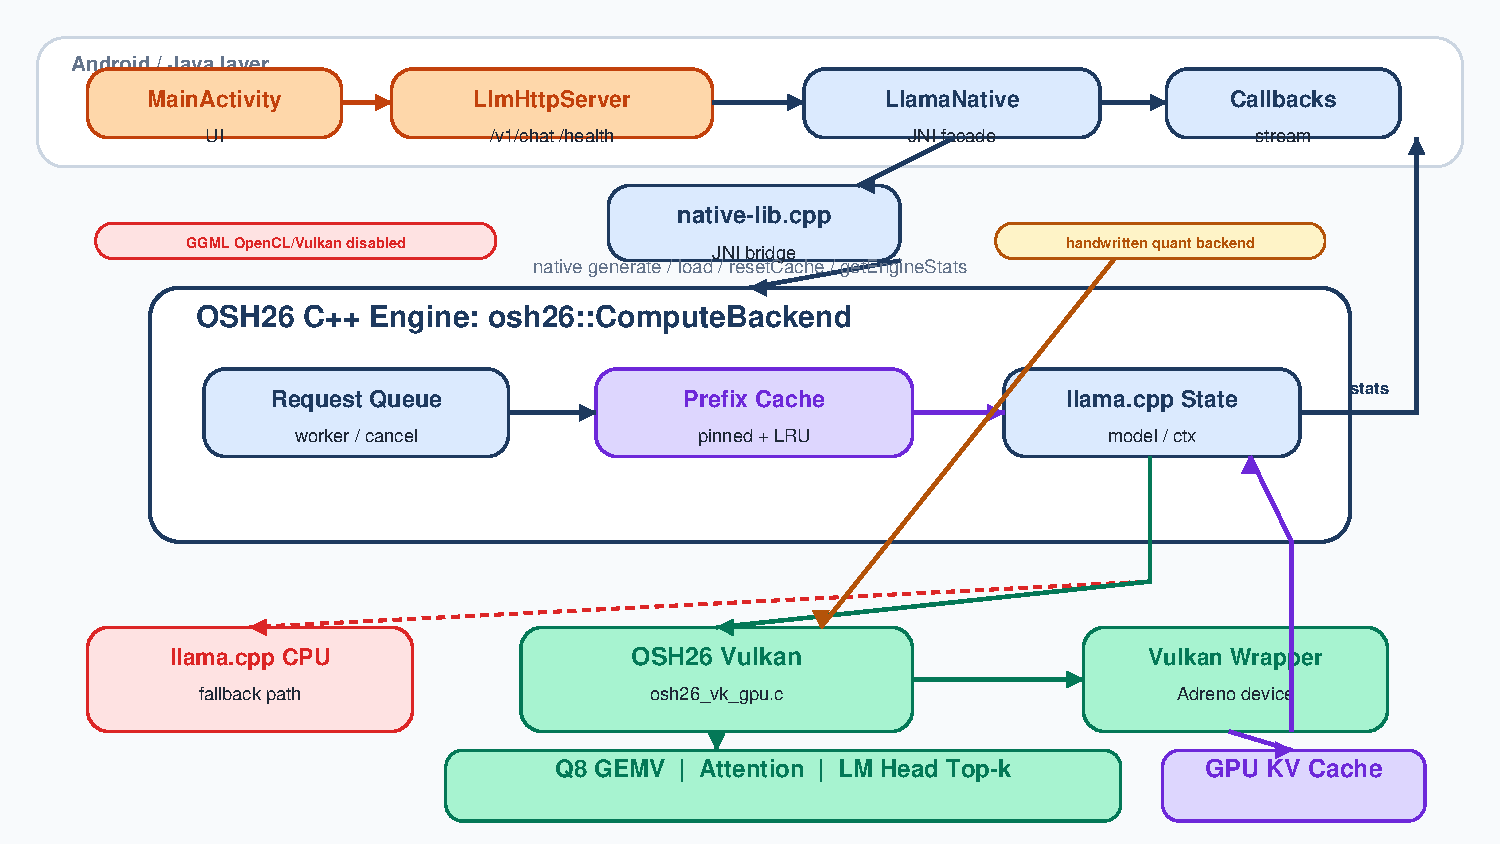
\includegraphics[width=\textwidth,height=0.84\textheight,keepaspectratio]{figures/llm-runtime-architecture.pdf}
  \end{center}
\end{frame}

\begin{frame}
  \frametitle{总体设计：CPU/GPU 分工与 KV Cache}
  \small
  移动端没有服务器级显存冗余。端侧 Runtime 需要显式管理哪些工作留在 CPU、哪些张量常驻 GPU，以及何时复用 KV。

  \vspace{0.4em}
  \scriptsize
  \begin{tabularx}{\textwidth}{p{0.20\textwidth}Y Y}
    \toprule
     & Runtime 实现 & 效果 \\
    \midrule
    控制面 / 数据面 & CPU 负责 tokenize、sampler、队列、cache policy；GPU 负责 Q8 投影、LM head、top-k & 控制逻辑保持灵活，密集计算留给 GPU \\
    工作集 & 活跃 prompt、Q8 权重、packed KV、临时 attention buffer & 避免不必要的 CPU/GPU 重复驻留 \\
    页缓存 & prefix cache page pool，按 token page 复用 K/V & 重复协议 prompt 不再完整 prefill \\
    \bottomrule
  \end{tabularx}
\end{frame}

\begin{frame}
  \frametitle{KV Cache：把上下文当虚拟内存管理}
  \begin{columns}[T,onlytextwidth]
    \begin{column}{0.48\textwidth}
      \begin{block}{Paged / Prefix 思路}
        \scriptsize
        \begin{itemize}
          \item 受 vLLM 启发：KV 不是一整块不可分割数组，而是可复用的 page。
          \item 固定系统提示词、工具协议、subagent 协议进入 pinned prefix。
          \item 普通对话使用 dynamic entry，采用LRU 回收策略。
        \end{itemize}
      \end{block}
    \end{column}
    % \begin{column}{0.48\textwidth}
    %   \scriptsize
    %   \begin{tabularx}{\textwidth}{p{0.40\textwidth}Y}
    %     \toprule
    %     指标 & 作用 \\
    %     \midrule
    %     命中状态 & 本次请求是否命中 prefix cache \\
    %     可复用 token & 可跳过 prefill 的前缀 token 数 \\
    %     Pinned entry & 固定协议前缀数量 \\
    %     碎片率 & page pool 的碎片状态 \\
    %     Restore 开销 & GPU 恢复 KV page 的时间 \\
    %     \bottomrule
    %   \end{tabularx}
    % \end{column}
  \end{columns}

  \vspace{0.35em}
  \footnotesize
  % 课程知识对应：KV Cache 类似页缓存；prefix key 类似页表索引；pinned entry 类似共享只读段；LRU / fragmentation / restore cost 决定长期运行稳定性。
\end{frame}

\begin{frame}
  \frametitle{Agent 专用优化：stateless subagent 的 pinned prefix}
  \small
  Action Fabric 会产生大量短生命周期 subagent：它们共享工具协议，但不应该继承完整聊天历史。我们把这个 workload 单独建模，而不是让它混在普通 chat cache 里。

  \vspace{0.35em}
  \scriptsize
  \begin{tabularx}{\textwidth}{p{0.24\textwidth}Y Y}
    \toprule
    场景 & 普通处理 & 我们处理 \\
    \midrule
    固定工具协议 & 每个 subagent 重新 prefill & \code{stateless\_subagent=true}，协议 prompt 进入 pinned prefix \\
    并发短任务 & 多份重复系统提示词挤占 KV & 一个 pinned entry 被多轮不同任务复用 \\
    普通聊天 & 可能和 subagent cache 混淆 & chat cache key 与 subagent cache key 分离 \\
    \bottomrule
  \end{tabularx}

  \vspace{0.55em}
  \scriptsize
  \begin{tabularx}{\textwidth}{p{0.26\textwidth}p{0.18\textwidth}p{0.18\textwidth}Y}
    \toprule
    模型 & Cold TTFT & Warm TTFT & 结论 \\
    \midrule
    0.6B-Q8\_0 & 1249.13 ms & 278.543 ms & TTFT 降低 77.7\% \\
    1.7B-Q8\_0 & 2787.45 ms & 610.29 ms & TTFT 降低 78.1\% \\
    \bottomrule
  \end{tabularx}
\end{frame}

\begin{frame}
  \frametitle{请求调度：模型服务也需要 OS 调度器}
  \begin{columns}[T,onlytextwidth]
    \begin{column}{0.52\textwidth}
      \small
      当前引擎提供 OpenAI-compatible HTTP 接口，但内部不是同步函数调用，而是带状态的 native request queue。

      \vspace{0.35em}
      \begin{itemize}
        \item \code{active\_request} 与 pending queue 分离。
        \item cancel/release 可作用于 active 与 queued request。
        \item \code{max\_pending\_requests} 提供背压。
        \item \code{prefix-aware-aging-v2} 兼顾 cache hit 与防饥饿。
      \end{itemize}
    \end{column}
    \begin{column}{0.44\textwidth}
      \scriptsize
      \begin{tabularx}{\textwidth}{p{0.38\textwidth}Y}
        \toprule
        理论 & 对应实现 \\
        \midrule
        短作业优先 & prefix hit 请求服务时间更短 \\
        Aging & cache miss 请求不会长期等待 \\
        临界区 & request state 使用锁与条件变量保护 \\
        背压 & pending queue 限制避免 UI/服务被拖垮 \\
        \bottomrule
      \end{tabularx}
    \end{column}
  \end{columns}
\end{frame}

\begin{frame}
  \frametitle{量化后端：面向 Adreno 的 Q8 数据通路}
  \scriptsize
  \begin{tabularx}{\textwidth}{p{0.23\textwidth}Y Y}
    \toprule
    模块 & 做法 & 实机意义 \\
    \midrule
    Q8\_0 权重常驻 & 使用 GGUF 原生 Q8\_0 tensor，减少重复展开与复制 & 给 8K context 和 1.7B 模型留下内存空间 \\
    W8A8 prefill & activation 动态 Q8，packed int8 dot，F32 accumulate & TTFT 主路径从 F16 prefill 7361.61 ms 降到 788.56 ms \\
    decode Q8 GEMV & \code{nt == 1} 走 subgroup \code{GEMV\_Q8} & 0.6B TPS +20.3\%，1.7B TPS +37.3\% \\
    GPU LM head & dot/top-k/merge 在 GPU 完成，只回传候选集 & 避免全词表 logits 搬回 CPU \\
    descriptor cache & 热路径 descriptor alloc 归零作为 gate & 防止系统调用开销吞掉 kernel 收益 \\
    \bottomrule
  \end{tabularx}

  \vspace{0.45em}
  \normalsize
  % 这不是“把 F32 kernel 换成 Q8 kernel”，而是把数据布局、驻留策略、候选集返回、submit/descriptor 成本和正确性 gate 一起重排。
\end{frame}

\begin{frame}
  \frametitle{优化路线：从能跑到可部署}
  \scriptsize
  \begin{tabularx}{\textwidth}{p{0.20\textwidth}Y Y}
    \toprule
    阶段 & git 历史中的工作 & 解决的问题 \\
    \midrule
    Android 闭环 & Android Studio、CPU 推理、OpenAI API、\code{configureBackend} & App 能调用模型服务 \\
    驱动探索 & 原生 Vulkan 加载成功但乱码；MNN Vulkan 基础设施；自研 compute shader & 证明原生路径不可控，转向可控后端 \\
    KV / prefill & 加 KV cache、LRU 管理、prefill 分块、GPU prefill、LM head 优化 & 降低 TTFT 与重复 prompt 成本 \\
    Q8 化 & 原生 Q8\_0、decode Q8、Q8\_0 单份权重驻留 & 降低内存与 decode latency \\
    扩展性 & 8K context、Qwen3-1.7B、消除 CPU 重复驻留 & 从 demo 模型走向可用端侧模型 \\
    Agent 化 & stateless subagent cache 策略 & 针对 Action Fabric 的真实 workload 优化 \\
    \bottomrule
  \end{tabularx}
\end{frame}

\begin{frame}
  \frametitle{实机性能与验证 gate}

  \small
  我们在红米K40真机（Adreno 650，12GB RAM）上跑Qwen3系列 0.6B-Q8\_0 和 1.7B-Q8\_0 模型，使用真实的Agent prompt序列，测量平均 TTFT、TPS
  \scriptsize
  \begin{tabularx}{\textwidth}{p{0.23\textwidth}p{0.18\textwidth}p{0.18\textwidth}Y}
    \toprule
    指标 & 0.6B-Q8\_0 & 1.7B-Q8\_0 & 说明 \\
    \midrule
    原有 TTFT median & 1249.13 ms & 2787.45 ms &  \\
    最新 TTFT median & 278.543 ms & 610.29 ms & decode Q8 GEMV 默认路径，分别提升 77.7\% 和 78.1\% \\
    原有 TPS median & 3.6718 & 1.9954 &  \\
    最新 TPS median & 6.8382 & 4.0614 & 相比旧 baseline，decode 速度分别提升 85.4\% 和 103.3\% \\
    % LM head median & 118.45 ms & 214.37 ms & GPU LM head + top-k candidate path \\
    % forward submits & 2 & 2 & 非 debug 正常路径，submit 成本受控 \\
    % descriptor alloc & 0 & 0 & 热路径 descriptor allocation 消除 \\
    % 8K context & \multicolumn{2}{c}{5488 user tokens / 43 chunks / valid output} & 证明不是只把 context 数字改大 \\
    \bottomrule
  \end{tabularx}

  \vspace{0.4em}
  \footnotesize
  % gate 不只看速度：还检查 token IDs reproducibility、logits sanity、attention fallback、top-k overlap、active request 泄漏和 debug correctness 隔离。
\end{frame}

\begin{frame}
  \frametitle{与 Action Fabric 合流：端侧 Agent OS}
  \small
  上层 Action Fabric 把 Agent 执行变成可校验、可调度、可恢复的 DAG；下层 OSH26 LLM Runtime 把本地模型变成可调度、可复用、可观测的系统服务。

  \vspace{0.4em}
  \scriptsize
  \begin{tabularx}{\textwidth}{p{0.24\textwidth}Y}
    \toprule
    Action Fabric 需求 & LLM Runtime 支撑 \\
    \midrule
    一次规划 Workflow & 本地低 TTFT 模型服务，减少云端依赖 \\
    大量短 subagent & stateless prompt + pinned prefix cache \\
    ready set 并发 & native queue、背压、prefix-aware aging \\
    失败恢复 & cancel、release、last error、token IDs、health telemetry \\
    上下文治理 & 普通 chat 与 subagent cache 隔离，避免上下文污染 \\
    \bottomrule
  \end{tabularx}

  \vspace{0.45em}
  \normalsize
  最终贡献：一个把模型、内存、驱动、调度、Action 执行统一起来的端侧 Agent Runtime。
\end{frame}
